\setchapterpreamble[u]{\margintoc}
\chapter{Statistical Approach to Drop Formation}
\labch{dropstat}


\section{Monte Carlo Approach}



% interested in long time dynamics as coalescences lead to larger drop sizes


\section{Millimeter Scale Ensembles}

We turn our attention towards slender ligaments whose widths are of the 
order of millimeters, a scale at which a multitude of fragmentation phenomena
\sidenote{Some examples of fragmentation at this length scale involve ligaments
generated by drop splashes on different substrates, secondary atomization of raindrops etc. 
}
take place, that are more or less visible to the naked eye.
In particular, for air-water systems (20 degree Celsius) the millimeter length 
scale corresponds to $Oh \sim O(10^{-2})$, where $Oh$ is the Ohnesorge number
based on the characteristic length scale of the ligaments. 
The characterization of our corrugated ligament setup using the set of adimensional
(e.g. \eqref{base_params}) numbers as discussed in the previous chapter is extended 
to describe our ensemble of ligaments, such that the exact set of parameters
correspond to a unique point in the phase space $\Phi$ of all possible combinations. 
The coalescences that intermittently occur after the initial breakup phase of 
the thread-like structure not only change the number of drops, but also impact the 
mean and dispersion of the size distribution due to the increase in the number of drops that 
are significantly larger than the width of the ligament of origin.   
This aspect of temporal dependence of the drop sizes corresponding to a particular ligament ensemble
is taken into account by specifying the time at which the statistics are recorded. 
Thus, our droplet ensembles associated with the millimeter scale ligaments can be uniquely described 
by a combination of the time $T$ and $\Phi_0$, where

\begin{align}
	\Phi_0 \equiv \left( Oh=10^{-2}, K=2\pi, \epsilon=1.0, \Lambda=50 \right). 
\end{align}

The definitions of the adimensional groups are identical to that used
in the previous chapter, hence are not repeated.
Statistical descriptions of the drop sizes are commonly carried out using
particular probability density functions (PDF) defined as follows 

\begin{align}
	\text{Gaussian : } \quad P\left( x ; \mu , \sigma \right) &= 
	\frac{1}{\sigma \sqrt{2\pi}} \textrm{exp}\left[-\frac{1}{2}\left(\frac{x - \mu}{\sigma}\right)^2\right] ,\\
	\text{Log-Normal : } \quad P\left( x ; \mu , \sigma \right) &= 
	\frac{1}{x \sigma \sqrt{2\pi}} \textrm{exp}\left[-\frac{1}{2}\left(\frac{\log x - \mu}{\sigma}\right)^2\right] ,\\
	\text{Gamma : } \quad P\left( x ; n,k \right) &= 
	\frac{k^{n}}{\Gamma(n)} x^{n-1} \textrm{exp}\left(-k x\right) , 
\end{align}

where $x$ is the variable (diameter, volume etc) in question. 
The Gamma distribution can be rearranged so that $x$ represents
the variable rescaled by its mean ($n / k$), which becomes 

\begin{align}
	P\left( x ; n \right) = \frac{n^{n}}{\Gamma(n)} x^{n-1} \textrm{exp}\left(-n x\right) . 
\end{align}

The rescaling of variable results renders the function dependent solely 
on the parameter $n$, identical to the form first used in \cite{vill_2}
to represent the distribution of the normalized diameter.  

Another important aspect to consider is the bin-width of the 
histograms used to construct the probability distributions. 
There are several choices regarding the criteria used to determine the optimal bin-width, 
taking into consideration the size, variability and skewness of the underlying data set. 
In in interest of simplicity, we restrict our focus to histograms with uniform bin-width. 
In order to ascertain the dependence (if any) of the distribution on the number of bins  
(uniform size), we use $4$ different estimators, the open source implementations of which
can be found in the Numpy library \sidecite{numpy}.
The simplest of the four estimators selects the number 
of bins as the square root of the sample size.
Another estimator is also based solely on the size of the dataset, 
but the number of bins scales as the cube root of the data size.  
A more robust estimator that takes into account the variability in the dataset
is the Freedman Diaconis estimator, in which the bin width is proportional to the 
inter quartile range, and inversely proportional to the cube root of the data size. 
Finally, we also use an improved version of the Sturges estimator, that performs 
well for non-normal datasets due to the fact that it takes into account the skewness. 

In the subsequent sections, we present a statistical picture of the drop sizes generated 
from our ligament ensemble $\Phi_0$, where the sample size is of the order of $64,000$.
The droplet data is primarily recorded on slow time scales, so that the data reflects 
a considerable amount of coalescences after the initial destabilization of the ligaments. 

\subsection*{Diameter Distributions}

Figures \ref{t1_dia_bins} and \ref{t2_dia_bins} illustrate the probability distributions
of droplet diameter corresponding to $T=15$ and $T=30$ respectively.  




\begin{figure*}
\centering
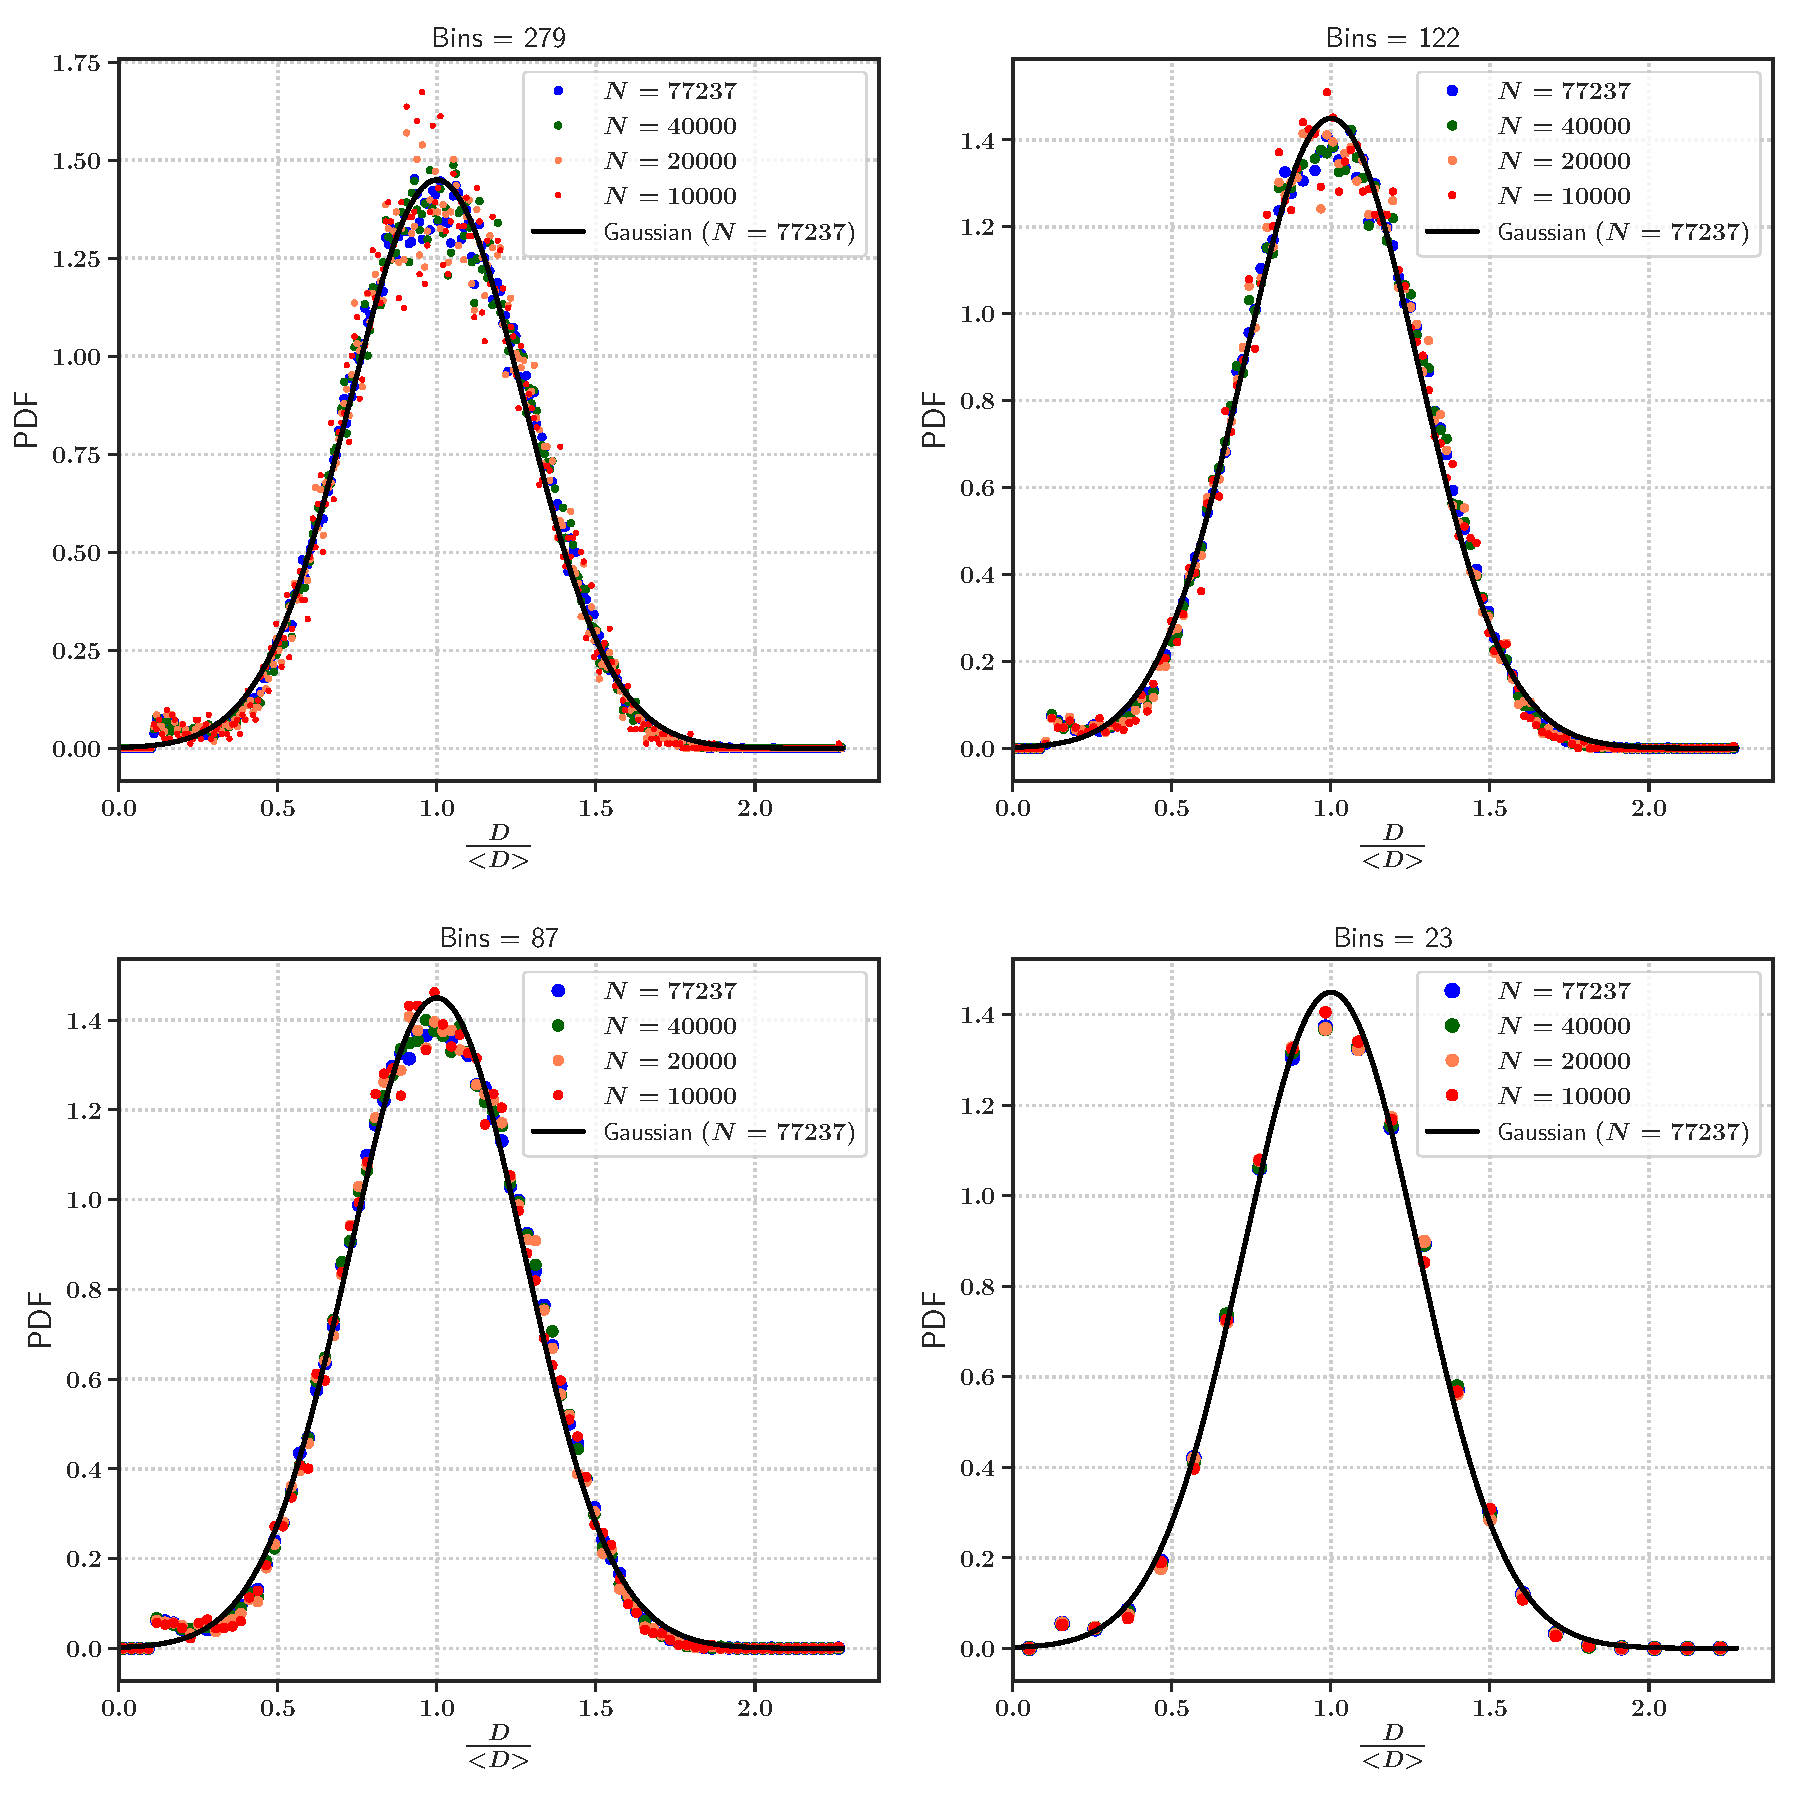
\includegraphics{plots/drop_stats/short_time_diameter_bins.pdf}
\caption{Probability distribution functions of the droplet diameter at time $T = 15$. 
The ensemble is characterized by $\Phi_0 \equiv \left( Oh = 10^{-2}, K = 2\pi , \varepsilon = 1.0 , \Lambda = 50 \right)$. 
The diameters are normalized by the mean of the corresponding sample.  
The distributions are generated using datasets corresponding to four different sample sizes, 
including four different choices of (uniform) bin width. 
The Gaussian functions are characterized by the mean and variance of the original dataset, 
hence they are plotted alongside the histograms instead of being fitted to the bin heights.
	}
\label{t1_dia_bins}
\end{figure*}

% long time scales


\begin{figure*}
\centering
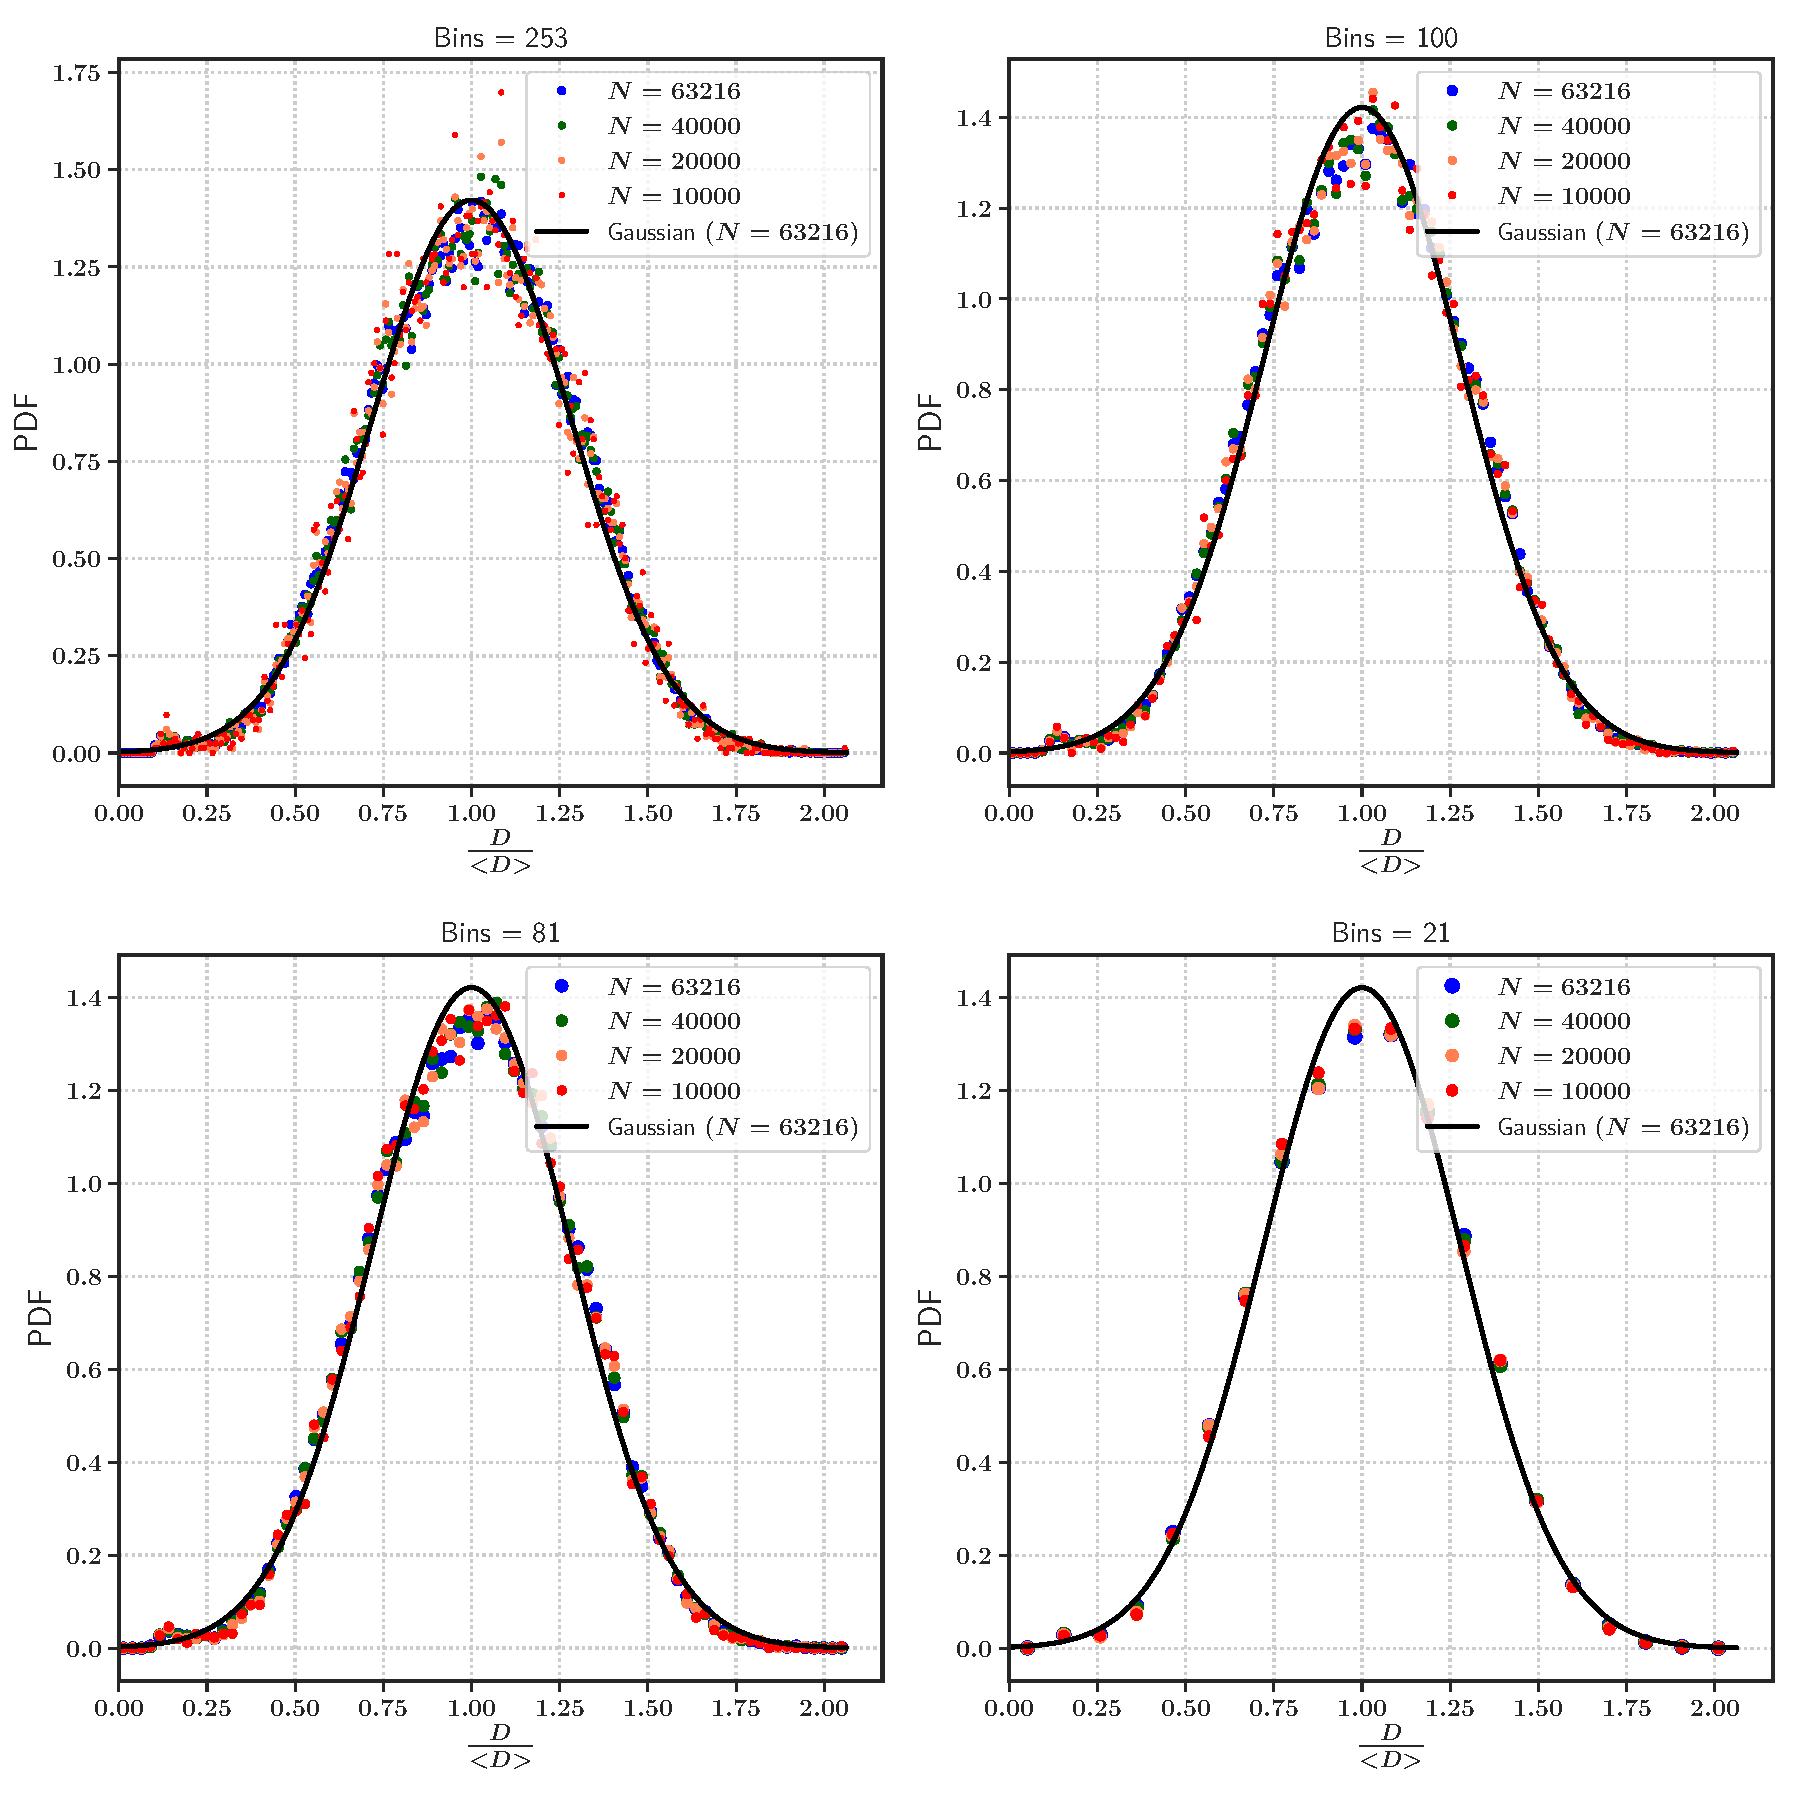
\includegraphics{plots/drop_stats/long_time_diameter_bins.pdf}
\caption{Probability distribution functions of the droplet diameter at time $T = 30$. 
The ensemble is characterized by $\Phi_0 \equiv \left( Oh = 10^{-2}, K = 2\pi , \varepsilon = 1.0 , \Lambda = 50 \right)$. 
The diameters are normalized by the mean of the corresponding sample.  
The distributions are generated using datasets corresponding to four different sample sizes, 
including four different choices of (uniform) bin width. 
The Gaussian functions are characterized by the mean and variance of the original dataset, 
hence they are plotted alongside the histograms instead of being fitted to the bin heights.
	}
\label{t2_dia_bins}
\end{figure*}

% PDF predictions of data at long times


\begin{figure*}
\centering
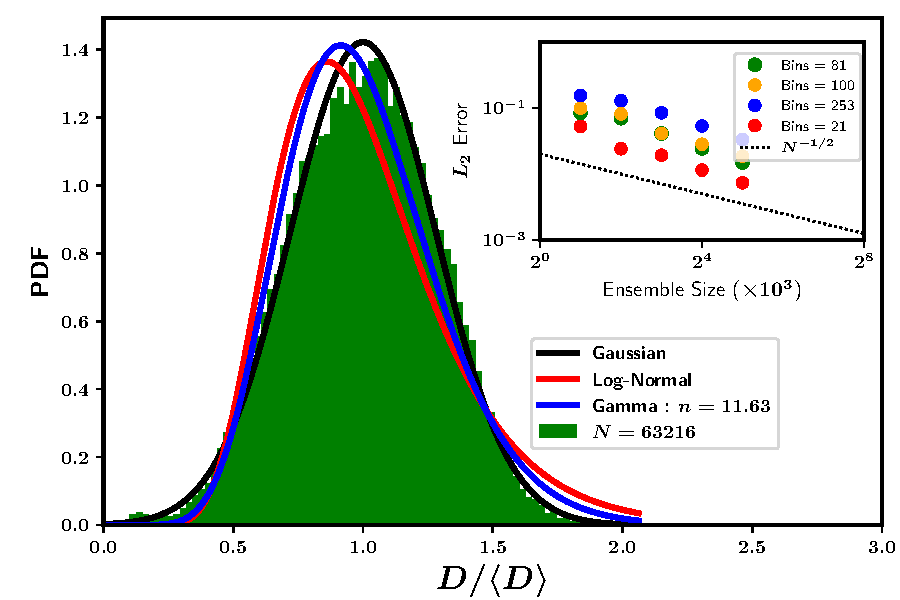
\includegraphics{plots/drop_stats/long_time_diameter_fits.pdf}
\caption{Probability distribution functions of the droplet diameter at time $T = 30$. 
The ensemble is characterized by $\Phi_0 \equiv \left( Oh = 10^{-2}, K = 2\pi , \varepsilon = 1.0 , \Lambda = 50 \right)$. 
The diameters are normalized by the mean of the corresponding sample.  
The distribution is generated using 81 bins of uniform size, represented in green.  
The Gaussian and Log-Normal functions are characterized by the mean and variance of the original dataset, 
therefore are plotted alongside the histogram, whereas, the Gamma function is fitted to the bin heights,
with $n= 11.63$ being the value corresponding to the best fit.
	}
\end{figure*}

% N^{-1/2} scaling of error 

% extrapolations of RP etc , limit of volume of largest drop

\subsection*{Volume Distributions}

% short time scale 


\begin{figure*}
\centering
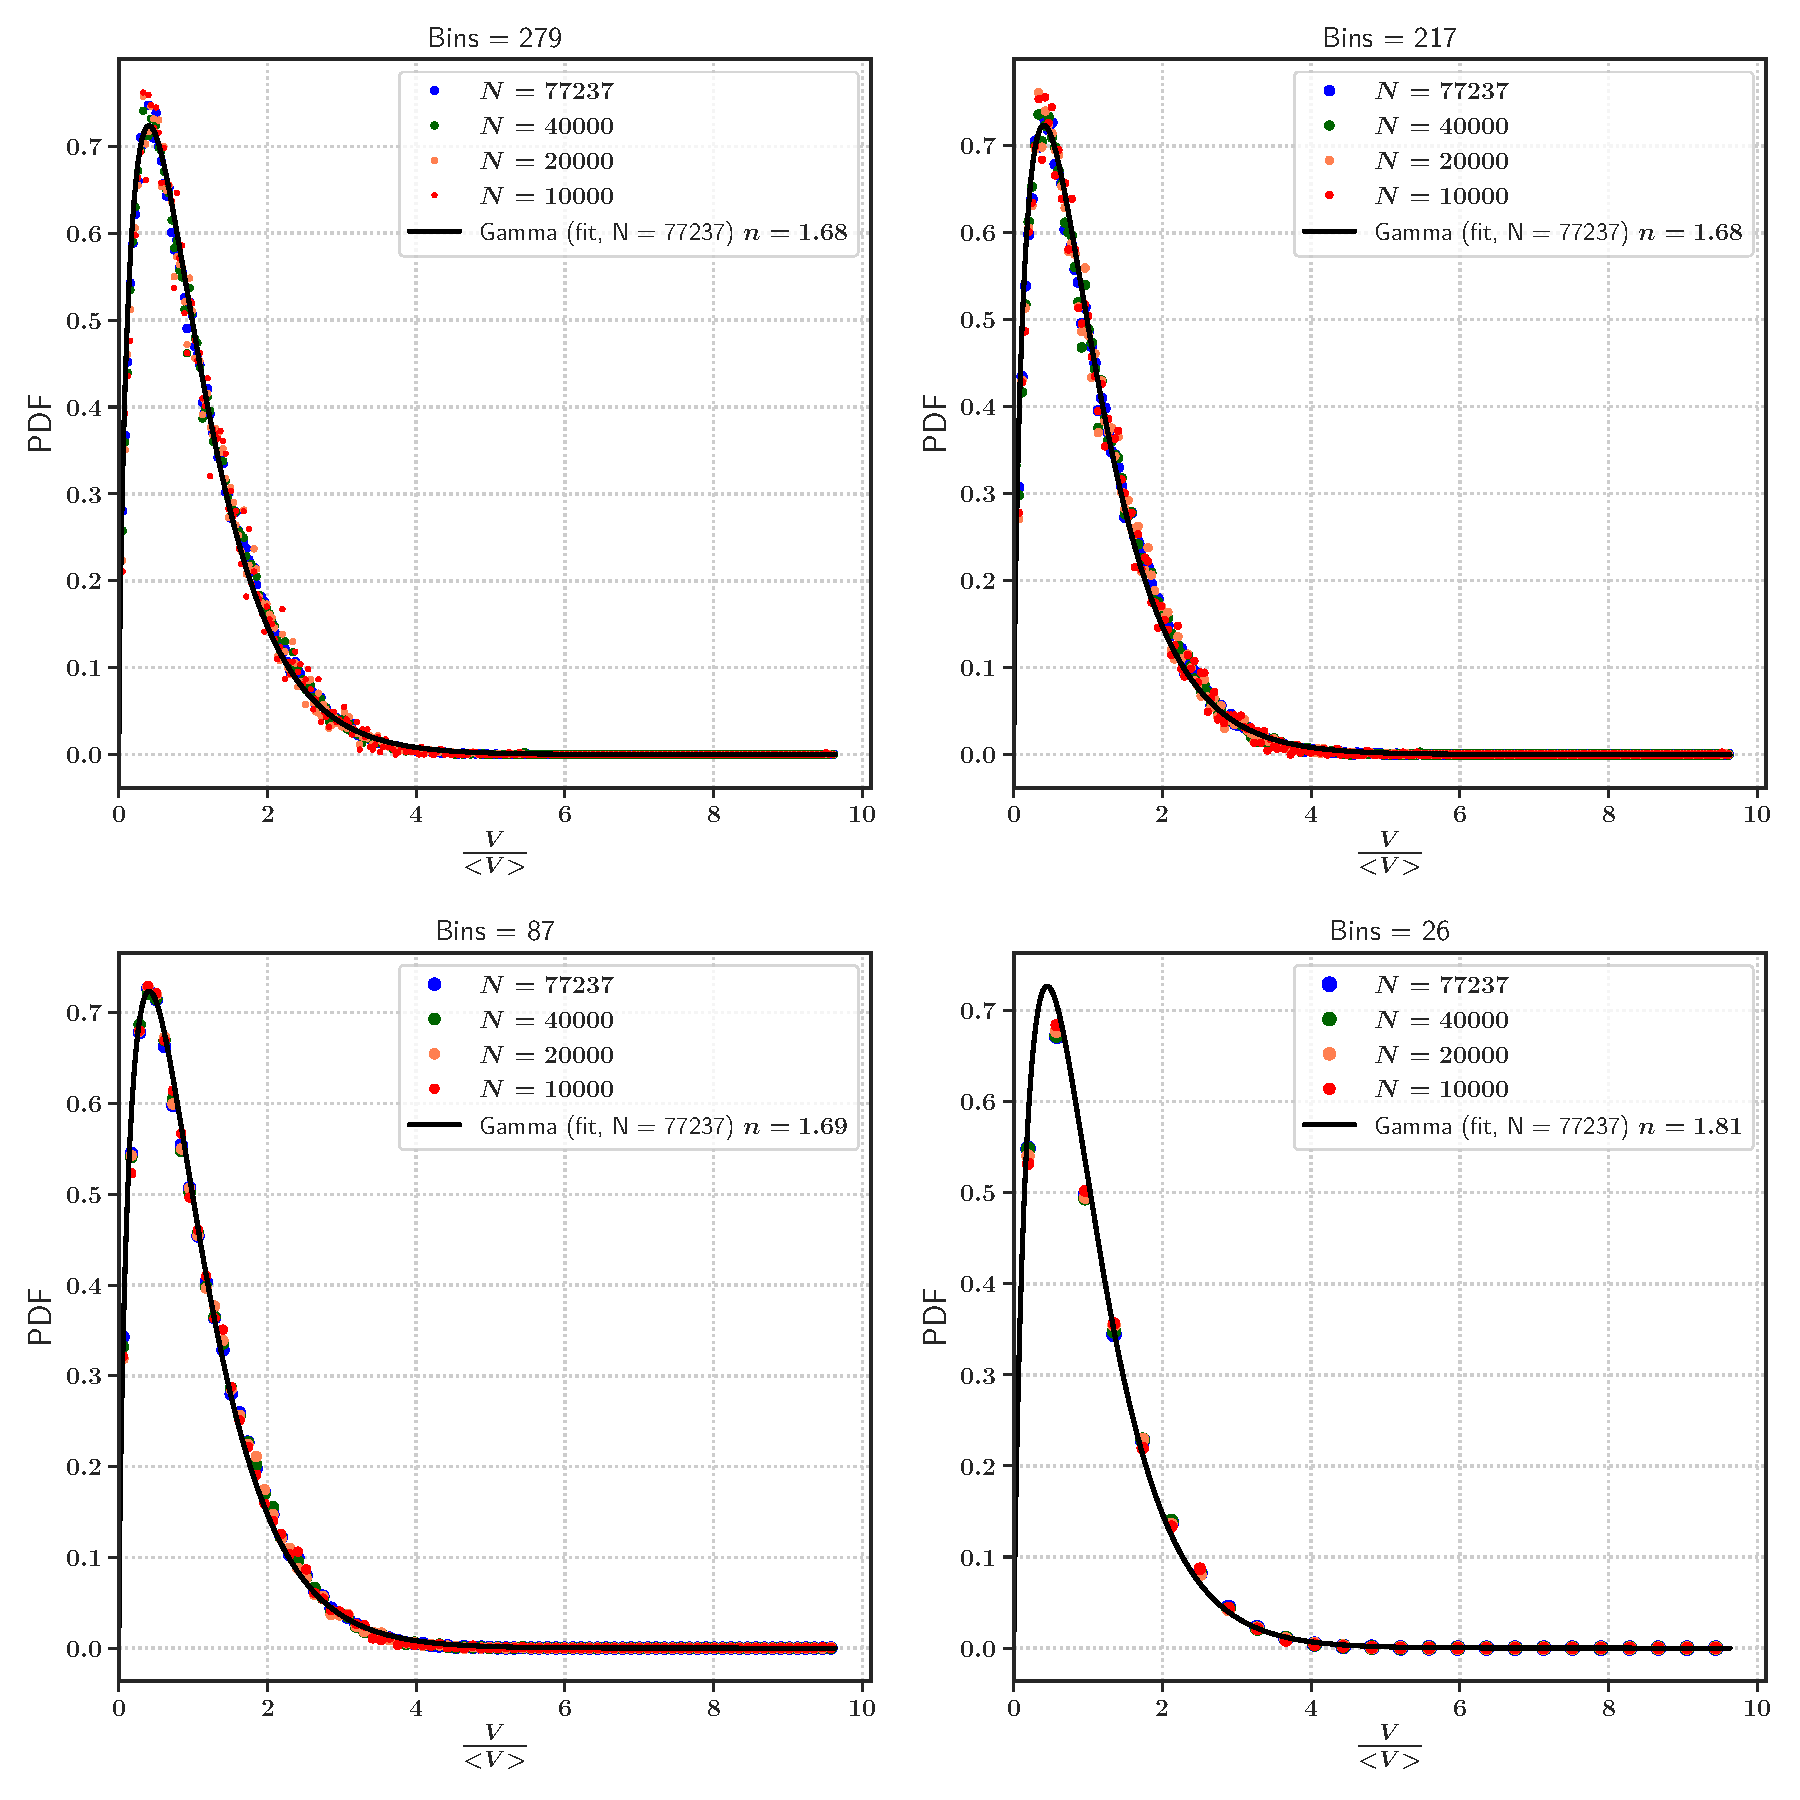
\includegraphics{plots/drop_stats/short_time_volume_bins.pdf}
\caption{Probability distribution functions of the droplet volume at time $T = 15$. 
The ensemble is characterized by $\Phi_0 \equiv \left( Oh = 10^{-2}, K = 2\pi , \varepsilon = 1.0 , \Lambda = 50 \right)$. 
The volumes are normalized by the mean of the corresponding sample.  
The distributions are generated using datasets corresponding to four different sample sizes, 
including four different choices of (uniform) bin width. 
The Gamma functions are characterized by the parameter $n$, the value of which is determined 
by that which provides the best (least-squares) fit to the corresponding bin heights.  
	}
\label{t1_vol_bins}
\end{figure*}



% long time scale


\begin{figure*}
\centering
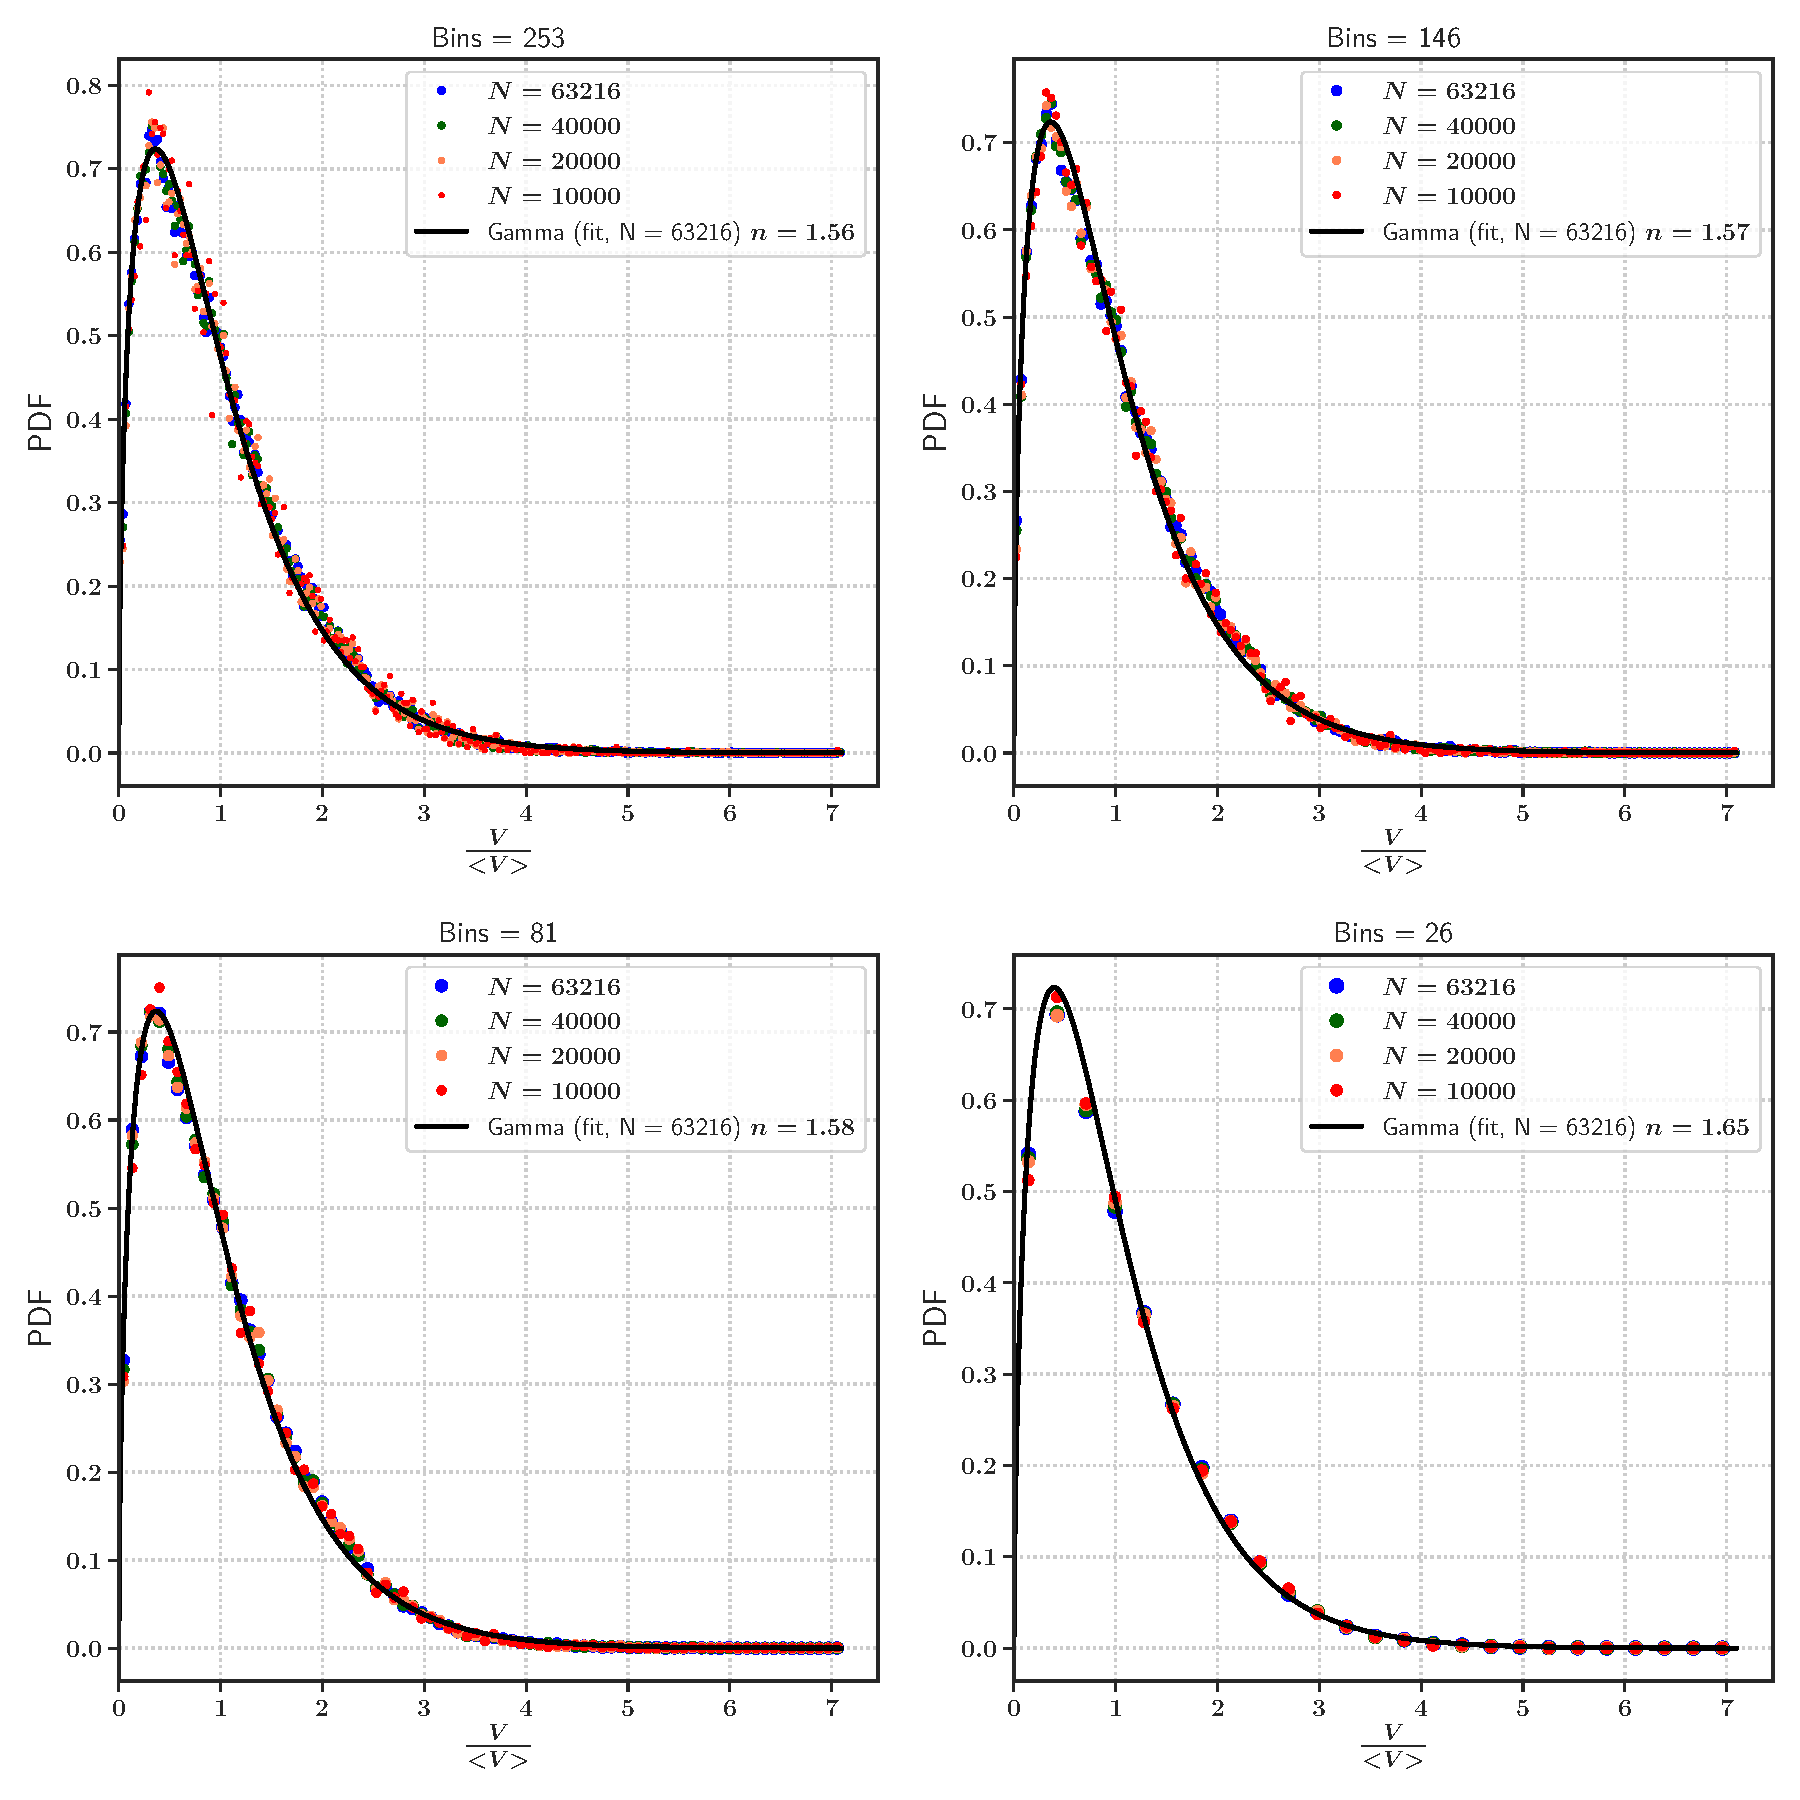
\includegraphics{plots/drop_stats/long_time_volume_bins.pdf}
\caption{Probability distribution functions of the droplet volume at time $T = 30$. 
The ensemble is characterized by $\Phi_0 \equiv \left( Oh = 10^{-2}, K = 2\pi , \varepsilon = 1.0 , \Lambda = 50 \right)$. 
The volumes are normalized by the mean of the corresponding sample.  
The distributions are generated using datasets corresponding to four different sample sizes, 
including four different choices of (uniform) bin width. 
The Gamma functions are characterized by the parameter $n$, the value of which is determined 
by that which provides the best (least-squares) fit to the corresponding bin heights.  
	}
\label{t2_vol_bins}
\end{figure*}


% PDF predictions of data at long times


\begin{figure*}
\centering
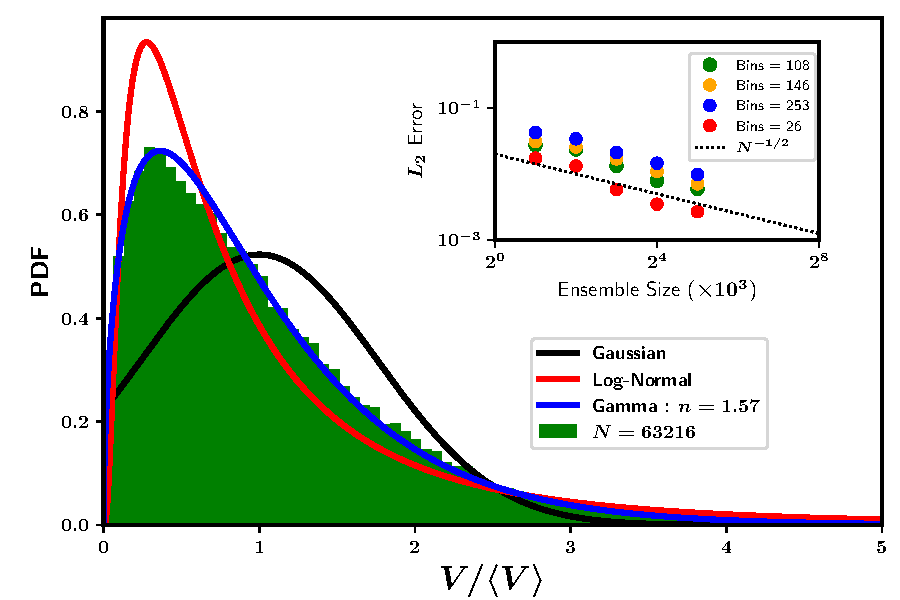
\includegraphics{plots/drop_stats/long_time_volume_fits.pdf}
\caption{Probability distribution functions of the droplet volume at time $T = 30$. 
The ensemble is characterized by $\Phi_0 \equiv \left( Oh = 10^{-2}, K = 2\pi , \varepsilon = 1.0 , \Lambda = 50 \right)$. 
The diameters are normalized by the mean of the corresponding sample.  
The distribution is generated using 108 bins of uniform size, represented in green.  
The Gaussian and Log-Normal functions are characterized by the mean and variance of the original dataset, 
therefore are plotted alongside the histogram, whereas, the Gamma function is fitted to the bin heights,
with $n= 1.57$ being the value corresponding to the best fit.
	}
\label{t2_vol_fits}
\end{figure*}

% N^{-1/2} scaling of error 


\subsection*{Influence of Corrugation Amplitude}

% temporal variation in drop size PDF's for low and high levels of corrugation

\begin{figure}
\centering
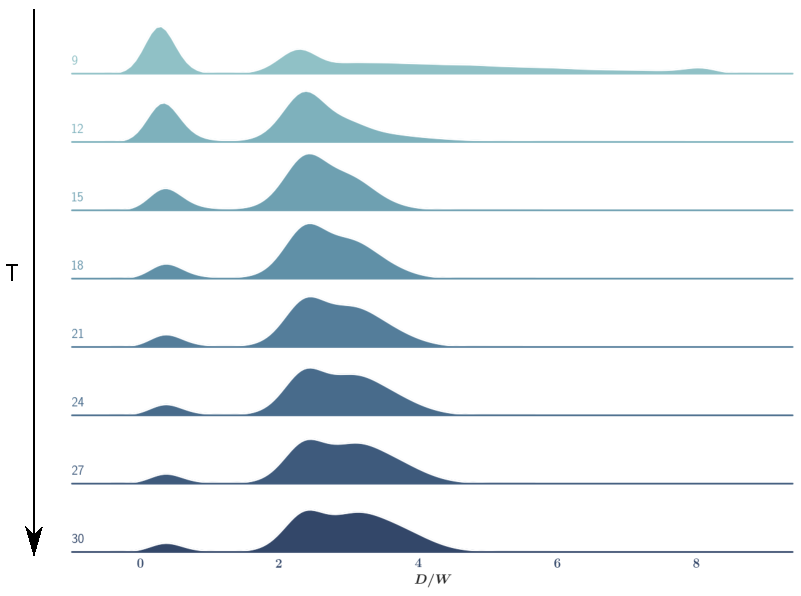
\includegraphics{plots/drop_stats/small_amp.pdf}
	\caption{\blindtext}
\label{tseries_small}
\end{figure}

\begin{figure}
\centering
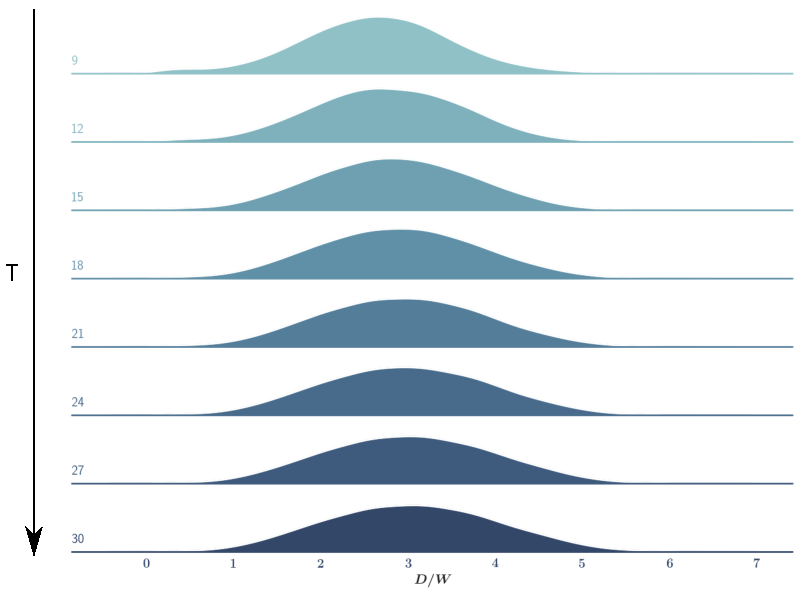
\includegraphics{plots/drop_stats/large_amp.pdf}
	\caption{\blindtext}
\label{tseries_large}
\end{figure}

% side by side comparison


\begin{figure*}
\centering
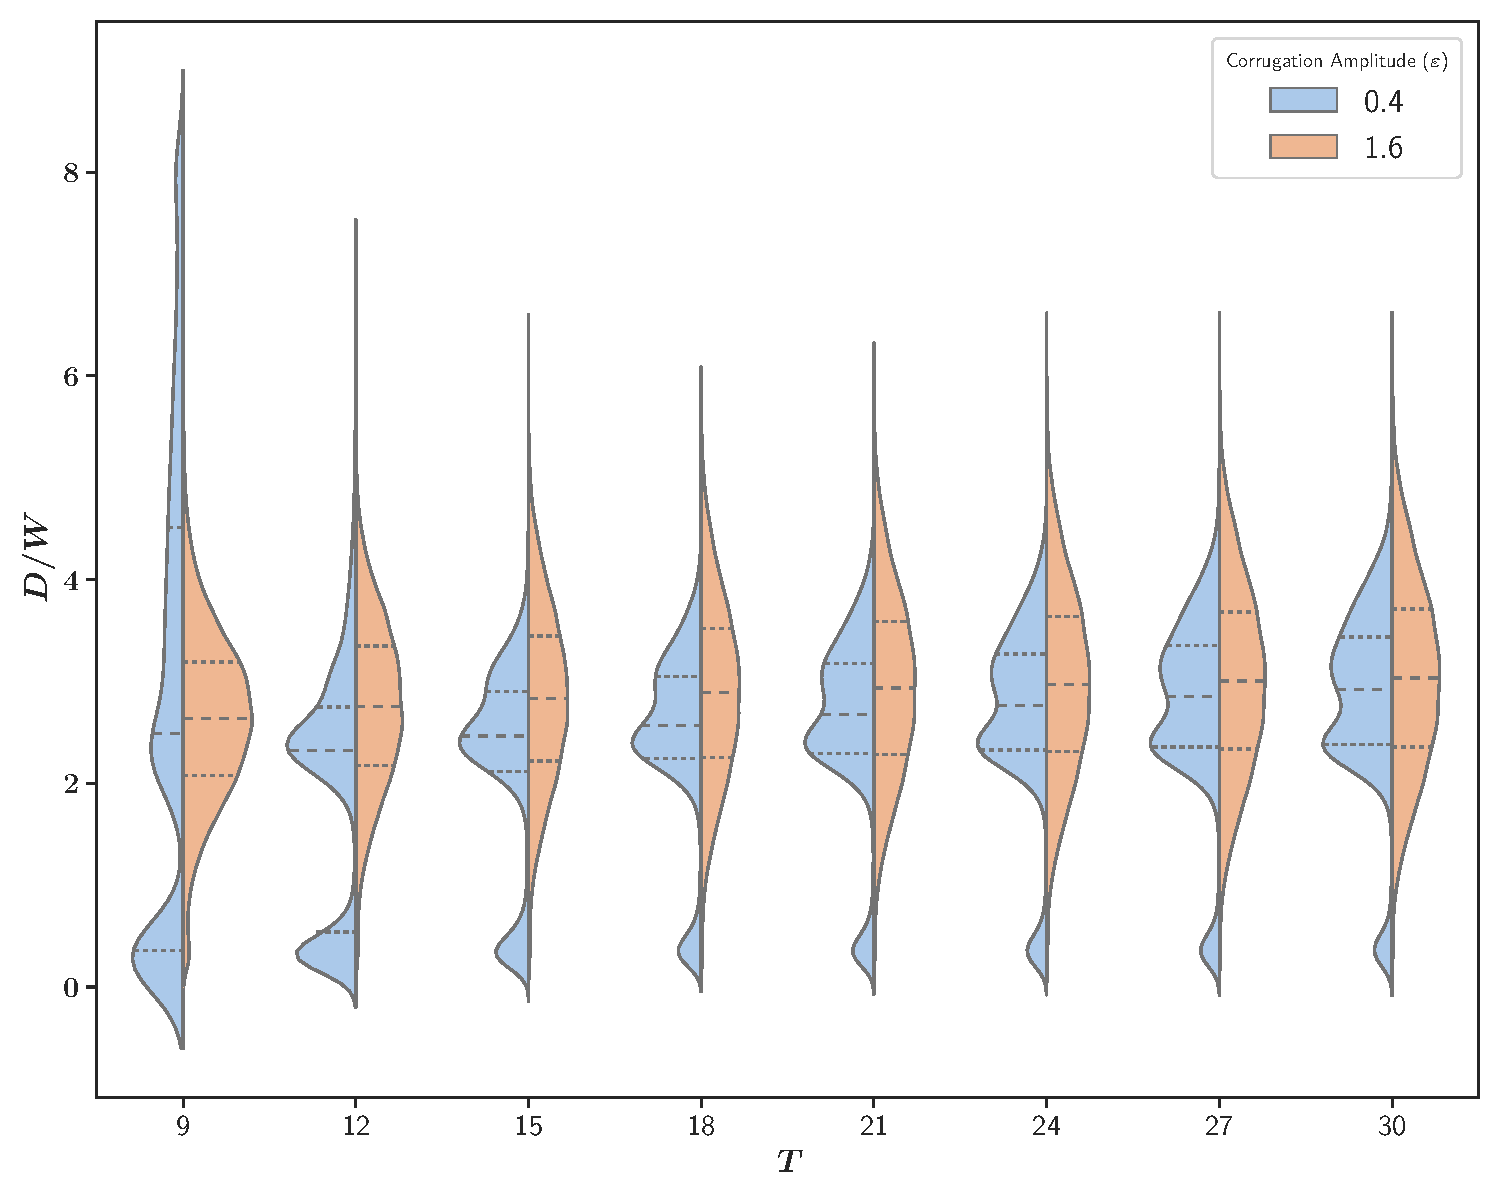
\includegraphics{plots/drop_stats/amp_dist_compare.pdf}
	\caption{\blindtext}
\label{tseries_comp}
\end{figure*}


\section{Description of Large Sizes}


% estimation of error with binomial distribution



% linear fitting, with and without uncertainty, full distribution and tail zoom  

% methodology to determine best fit

\begin{figure}
\centering
	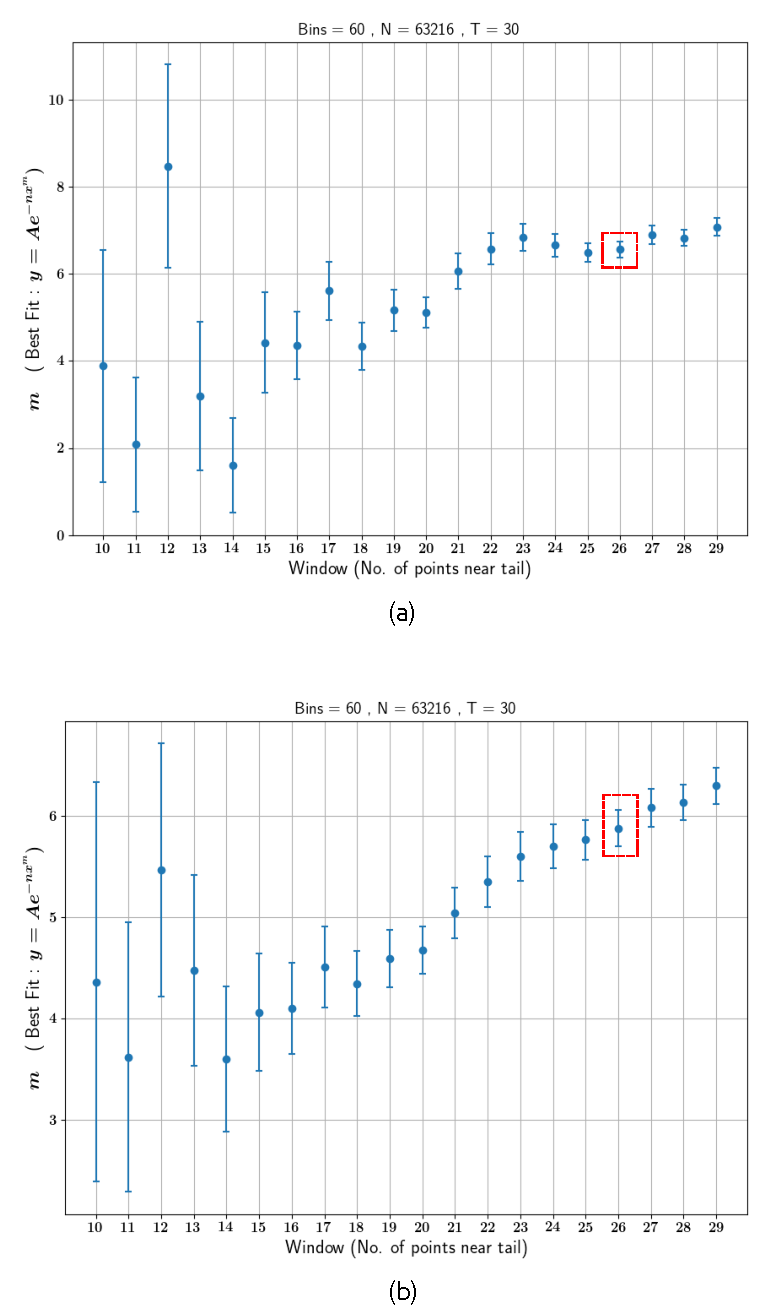
\includegraphics{plots/drop_stats/determine_fit_linear.pdf}
	\caption{\blindtext}
\label{determine_linear}
\end{figure}


% without uncertainty

\begin{figure}
\centering
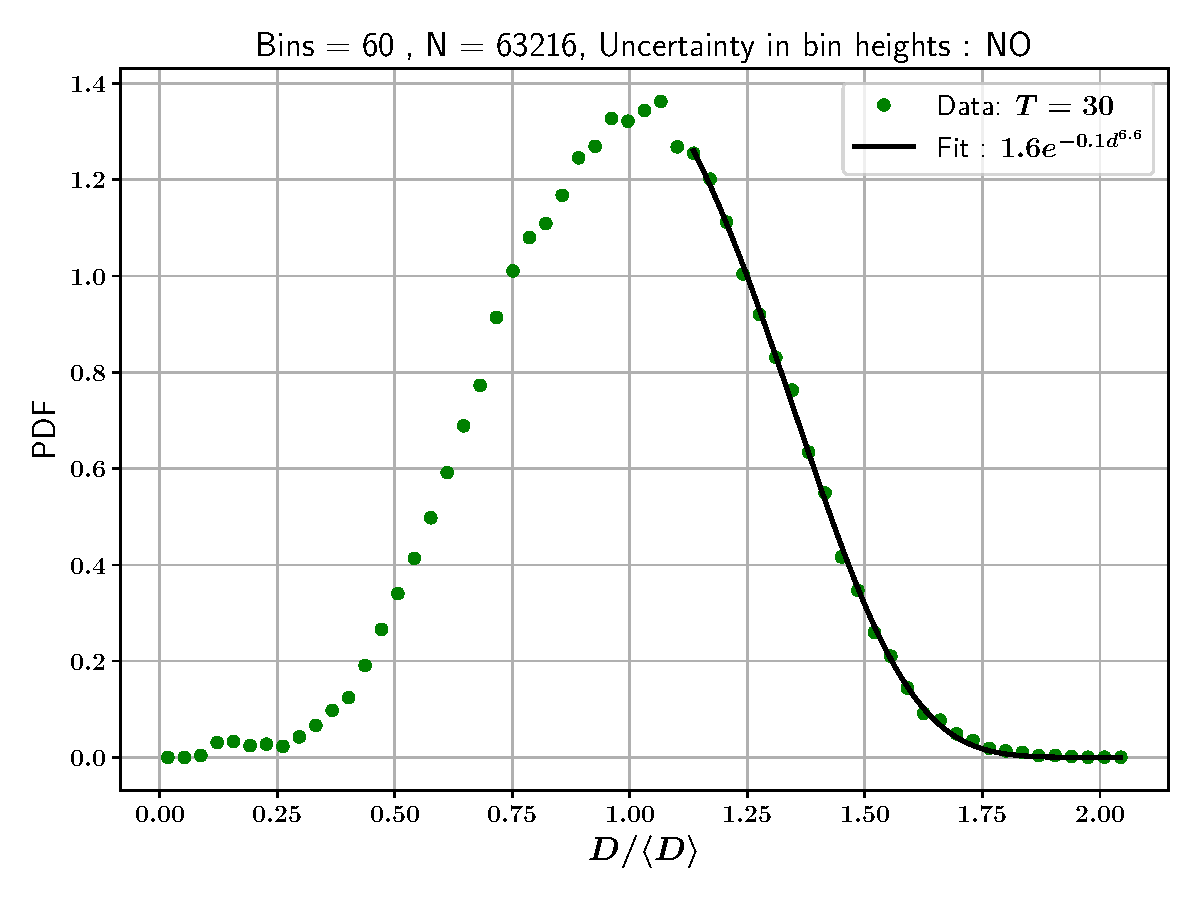
\includegraphics{plots/drop_stats/linear_tail_fit_uncertainty_no.pdf} \\
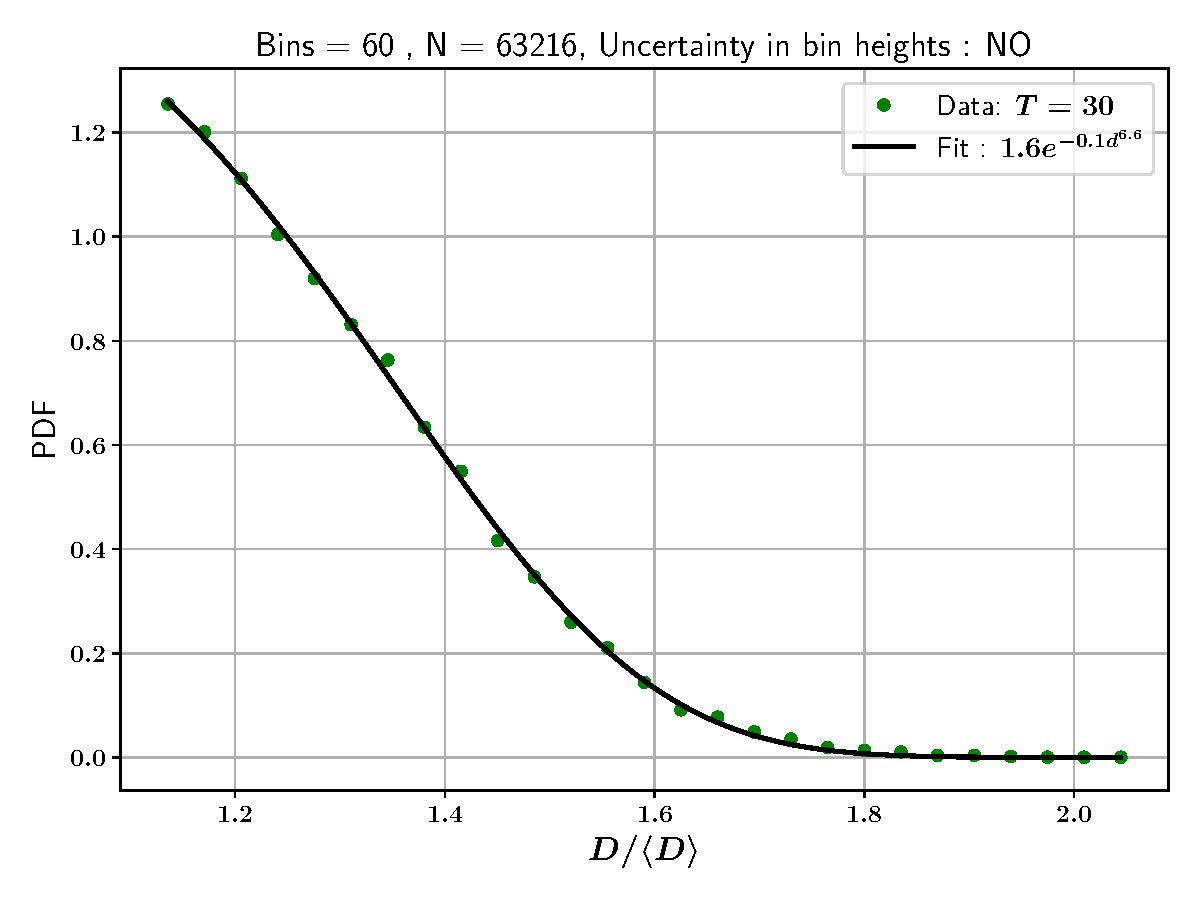
\includegraphics{plots/drop_stats/linear_zoom_tail_fit_uncertainty_no.pdf} \\ 
\caption{\blindtext}
\label{linear_fits_wo}
\end{figure}

% with uncertainty

\begin{figure}
\centering
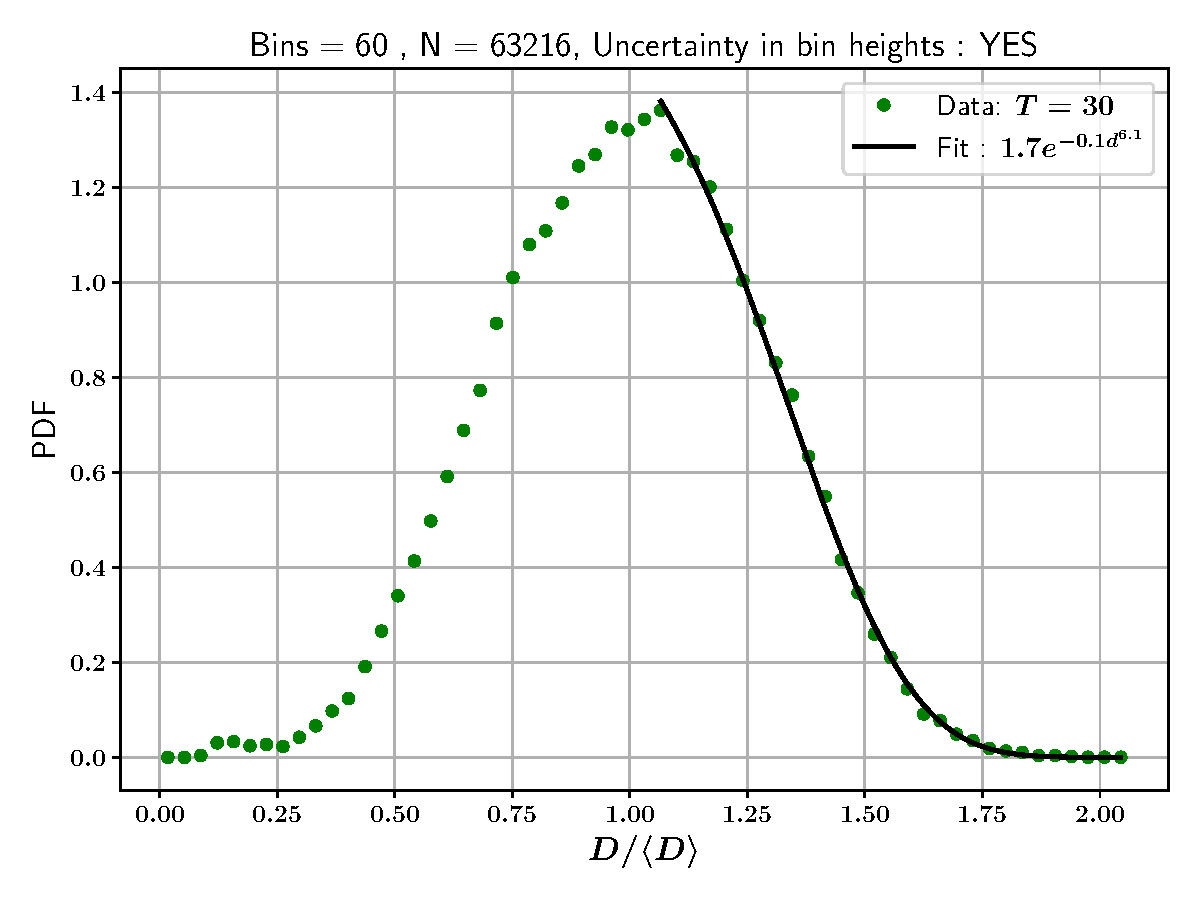
\includegraphics{plots/drop_stats/linear_tail_fit_uncertainty_yes.pdf} \\
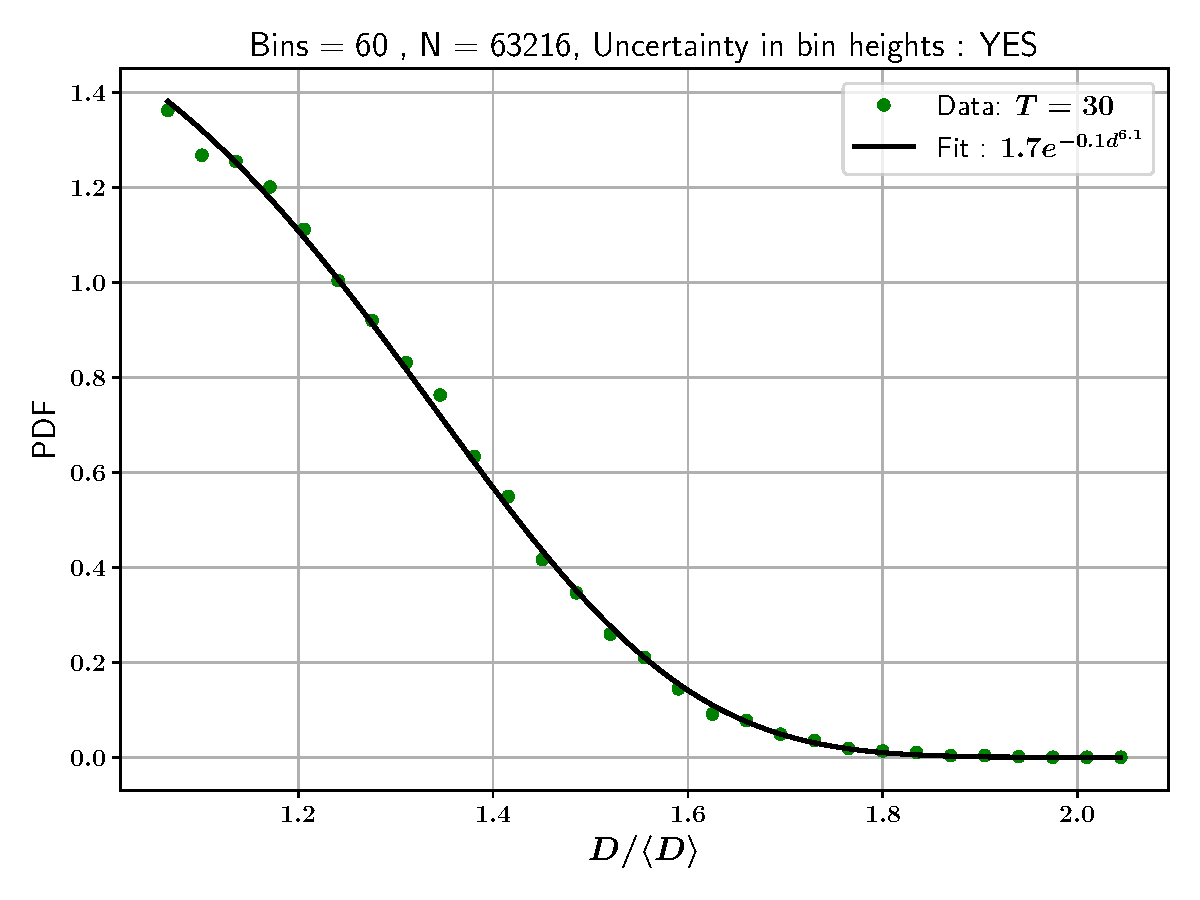
\includegraphics{plots/drop_stats/linear_zoom_tail_fit_uncertainty_yes.pdf} \\ 
\caption{\blindtext}
\label{linear_fits_with}
\end{figure}


% log(log) vs log fitting, with and without uncertainty, full distribution and tail zoom  

% methodology to determine best fit

\begin{figure}
\centering
	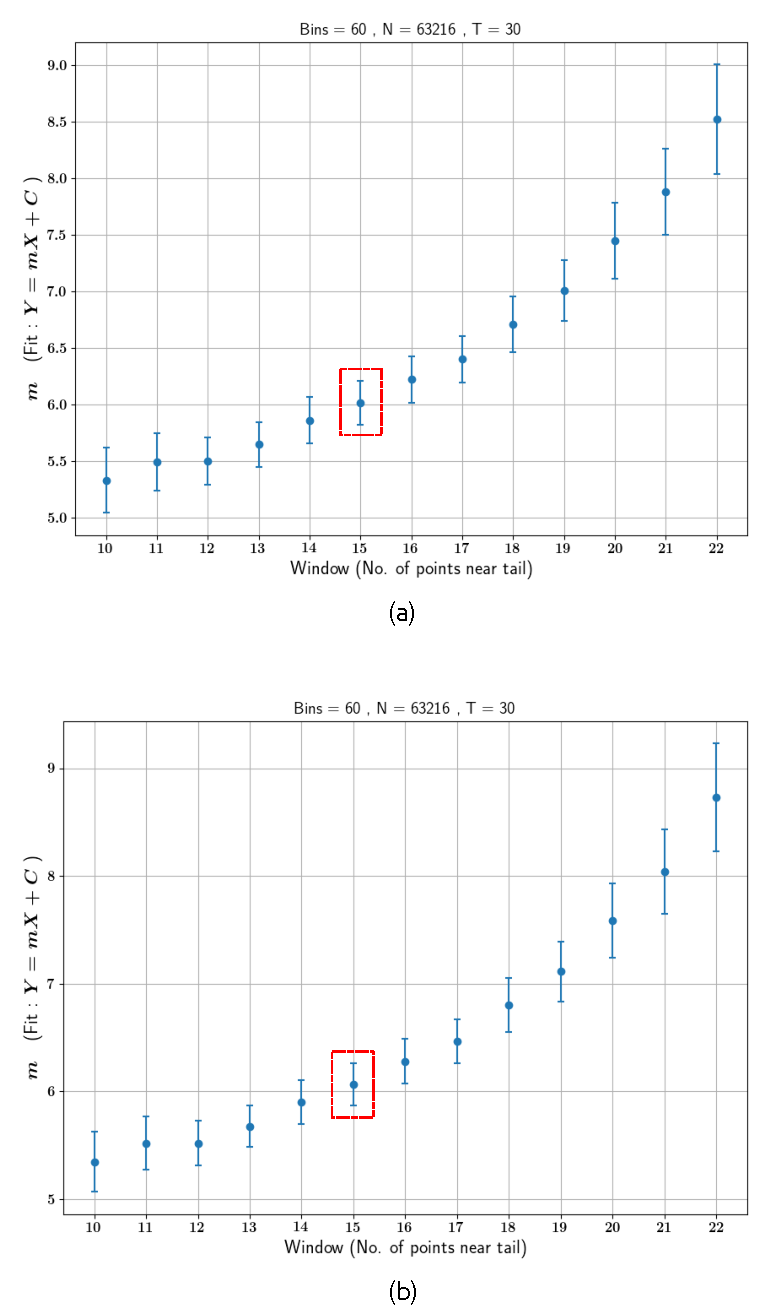
\includegraphics{plots/drop_stats/determine_fit_log.pdf}
	\caption{\blindtext}
\label{determine_log}
\end{figure}

% without uncertainty

\begin{figure}
\centering
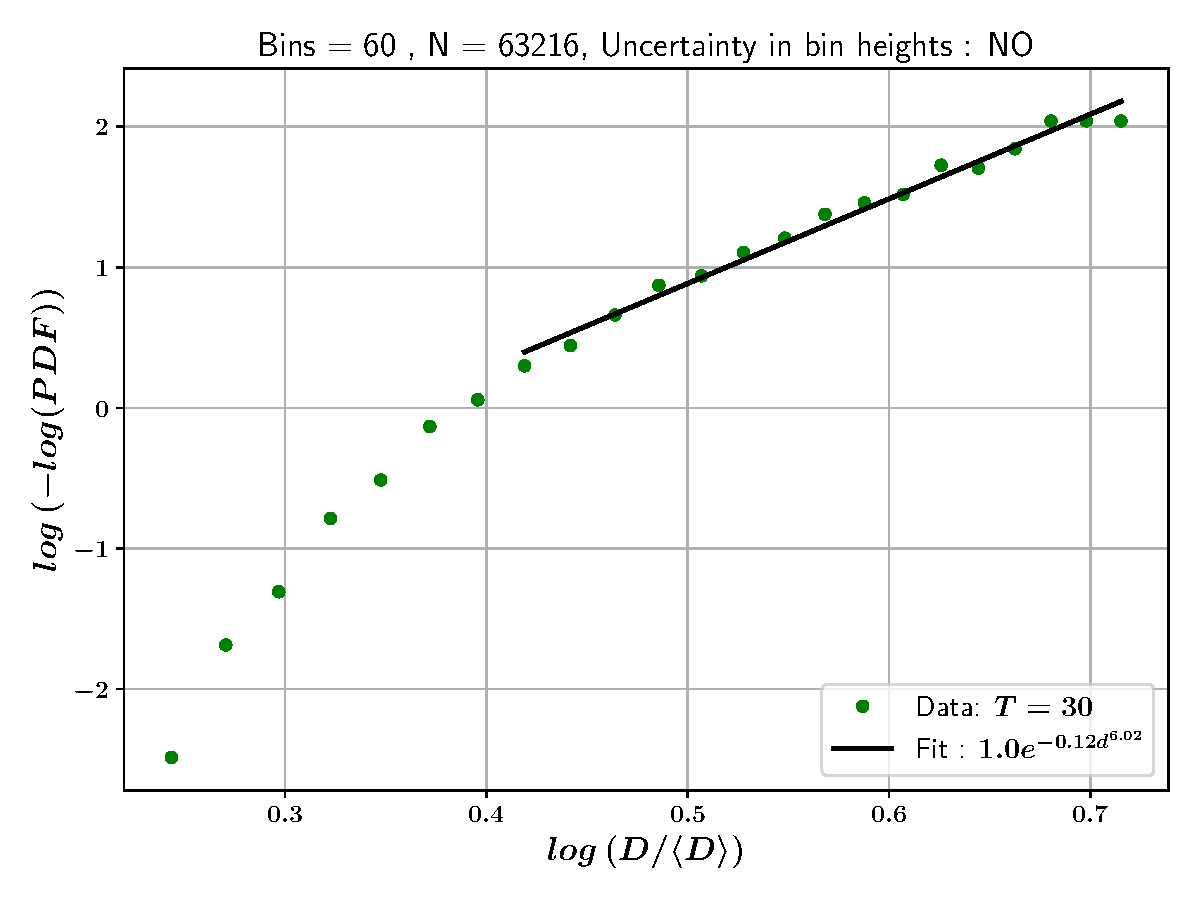
\includegraphics{plots/drop_stats/log_tail_fit_uncertainty_no.pdf} \\
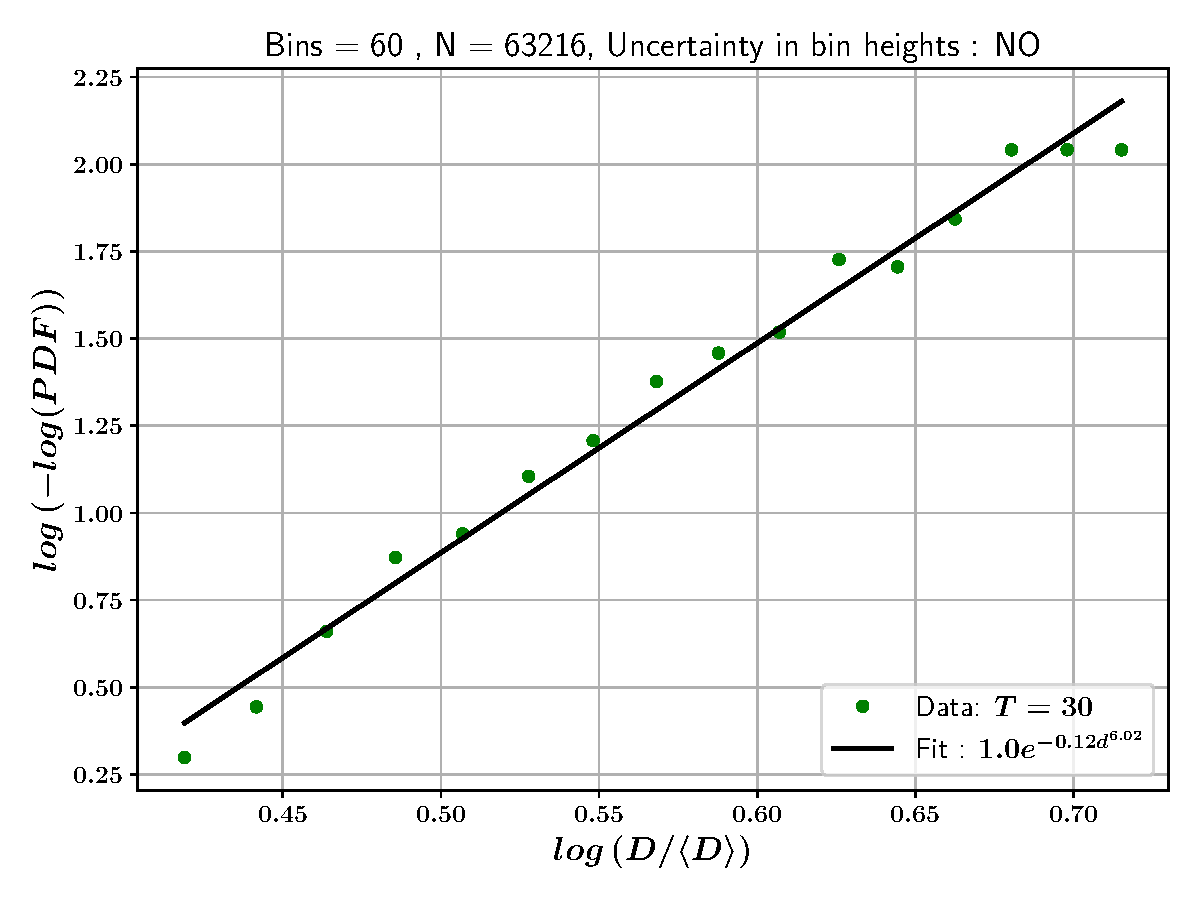
\includegraphics{plots/drop_stats/log_zoom_tail_fit_uncertainty_no.pdf} \\ 
\caption{\blindtext}
\label{log_fits_wo}
\end{figure}


% with uncertainty

\begin{figure}
\centering
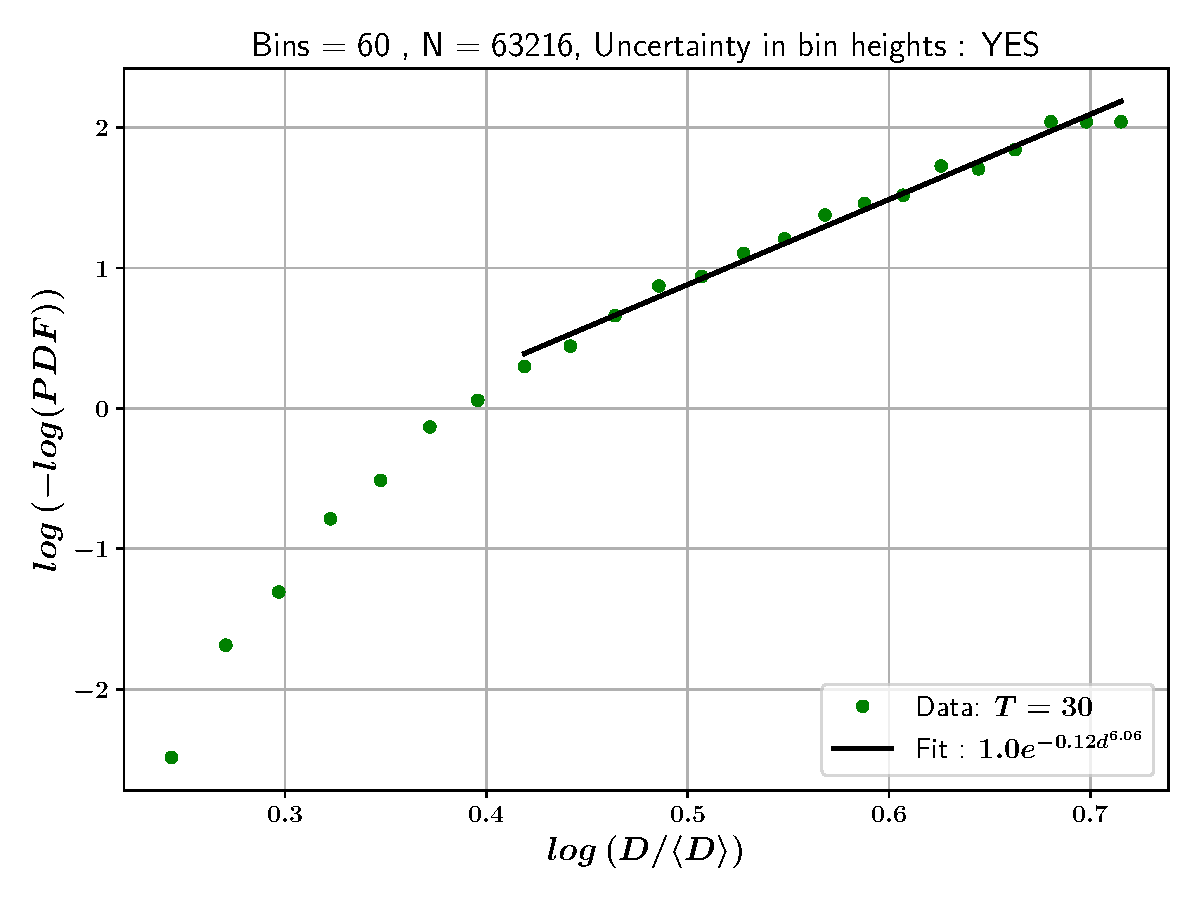
\includegraphics{plots/drop_stats/log_tail_fit_uncertainty_yes.pdf} \\
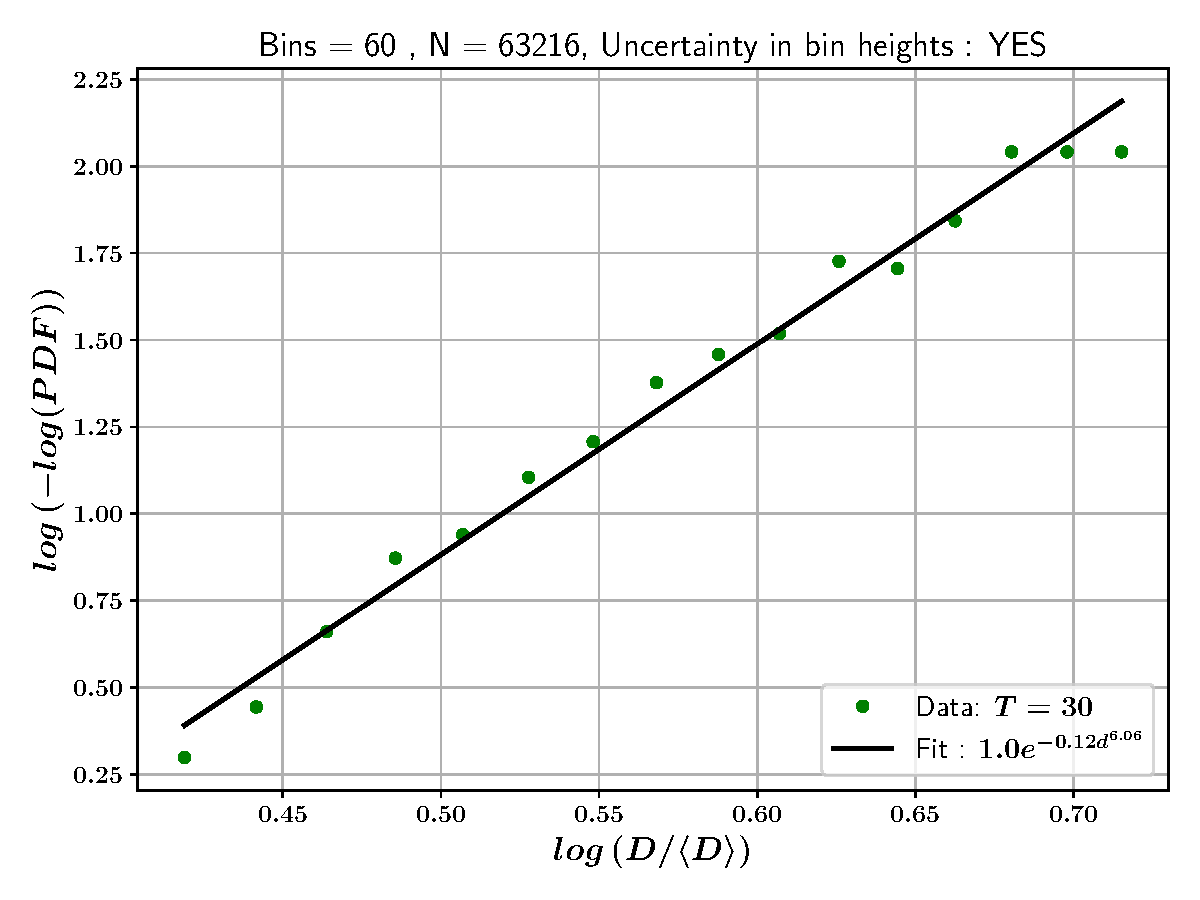
\includegraphics{plots/drop_stats/log_zoom_tail_fit_uncertainty_yes.pdf} \\ 
\caption{\blindtext}
\label{log_fits_with}
\end{figure}

\subsection*{Weakly Non-Linear Theory}



% stephane's predictions and verifications


